\graphicspath{{./figures}}

\section{Ground Station}
A block diagram of the system components for the ground station is shown in Figure \ref{fig:gs_system}.

\begin{figure}[!htb]
  \centering
  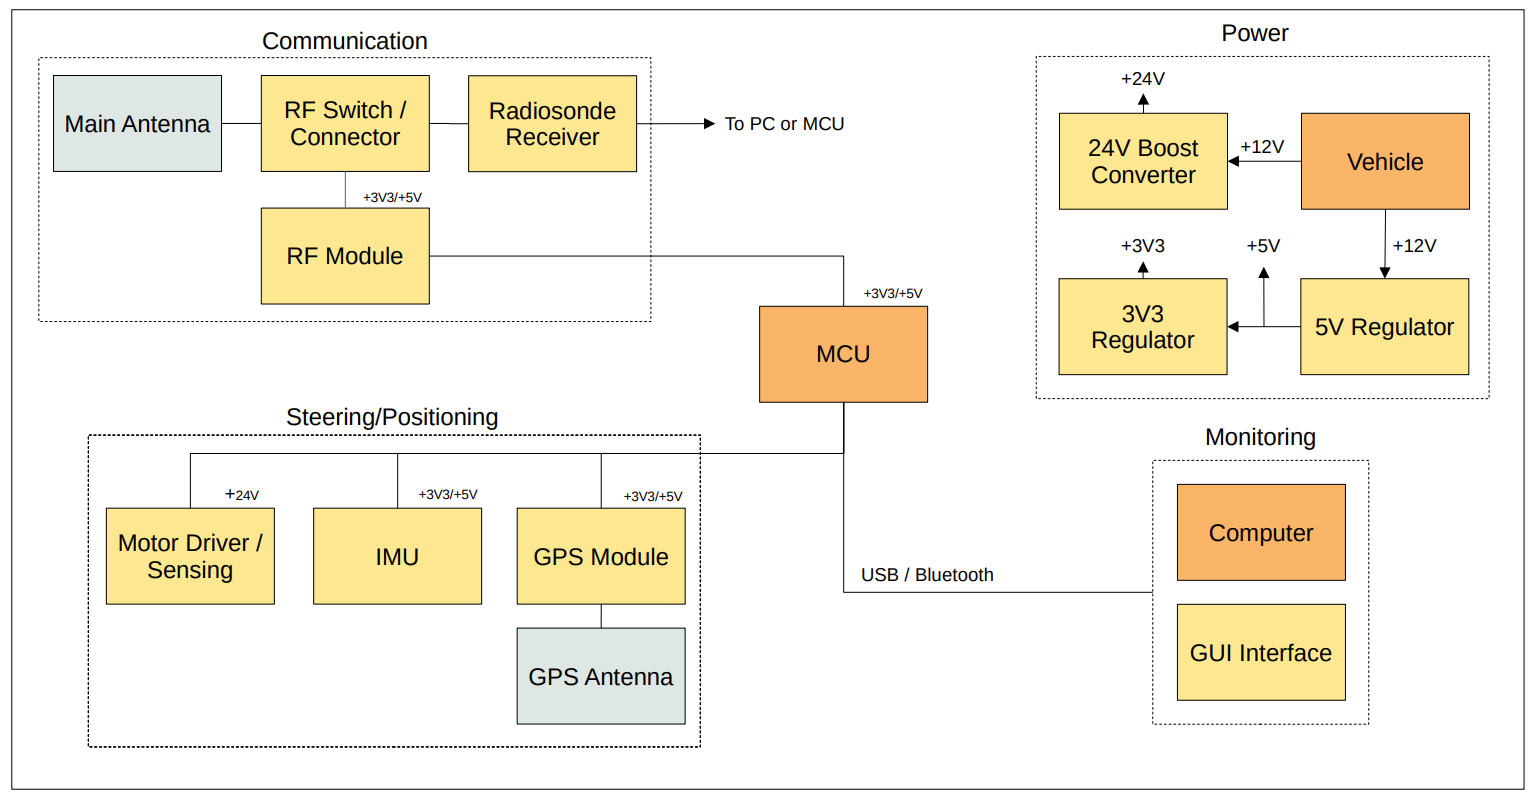
\includegraphics[width=0.95\textwidth]{gs_system}
  \caption{Groud Station System Diagram}
  \label{fig:gs_system}
\end{figure}

\subsection{Power}
The power section consists of two linear regulators, as well as a boost converter. The existing antenna mount has two \textit{NEMA 17 4218S-15} stepper motors, which will be used to steer the ground station in the direction of the satellite. These motors are ideally powered from +24V, and therefore a boost converter will be used to step up the voltage from the car's voltage of +12V. Further, +5V and +3V3 regulators will be included to power both the MCU and any other ICs, depending on their required voltage levels. Linear regulators were selected, due to their simplicity and the lack of any specific system-wide efficiency requirements.

\subsection{Communication}
The communication section consists of the main antenna, as well as the RF control circuitry and connectors. The \textit{RF Switch/Connector} is provided to allow the antenna to be shared between the custom and radiosonde communication links. Initially, a connector will be used for prototyping. Then, if time allows, a dedicated RF switch will be included, which will allow for the MCU to control the antenna connection. Both the RF module and the radiosonde receiver will connect through the RF switch/connector and to the antenna. The radiosonde will either connect to the PC (e.g. if an SDR dongle is used) or to the MCU (if a dedicated receiver is used).

\subsection{Steering and Positioning}\label{sec:gs_steering_positioning}
\begin{figure}[!htb]
    \centering
    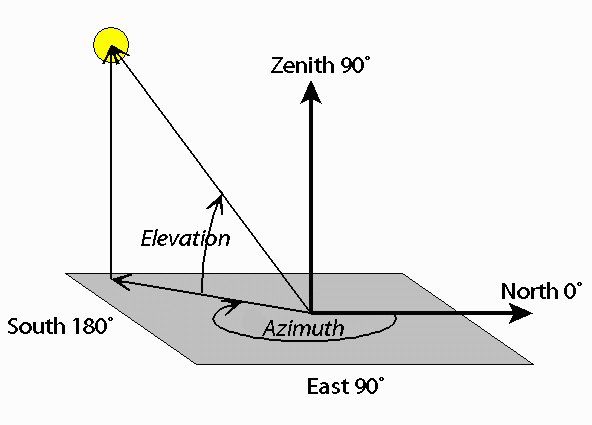
\includegraphics[width=0.4\textwidth]{az_elevation}
    \caption{Azimuthal and Elevation Visualization \cite{site-azElevationVisual}}
    \label{fig:az_elevation}
\end{figure}

Generally, the orientation of a ground station's antenna is described by both an azimuthal and an elevation angle, as in Figure \ref{fig:az_elevation}. The existing two-axis antenna mount is shown in Figure \ref{fig:antennaMount}. Since the antenna platform moves relative to the base (where the PCB is mounted), this relative angle needs to be known. Two options to do this are considered:
\begin{enumerate}
    \item \textit{Open-loop}. The base's absolute orientation is measured/known, and the platform's relative orientation is calibrated and calculated/looked up based on the stepper motor positions.
    \item \textit{Closed-loop}. The platform's absolute orientation is measured in real-time, and this information is fed back into the motor's control system to point the platform correctly.
\end{enumerate}

\begin{figure}[!htb]
    \centering
    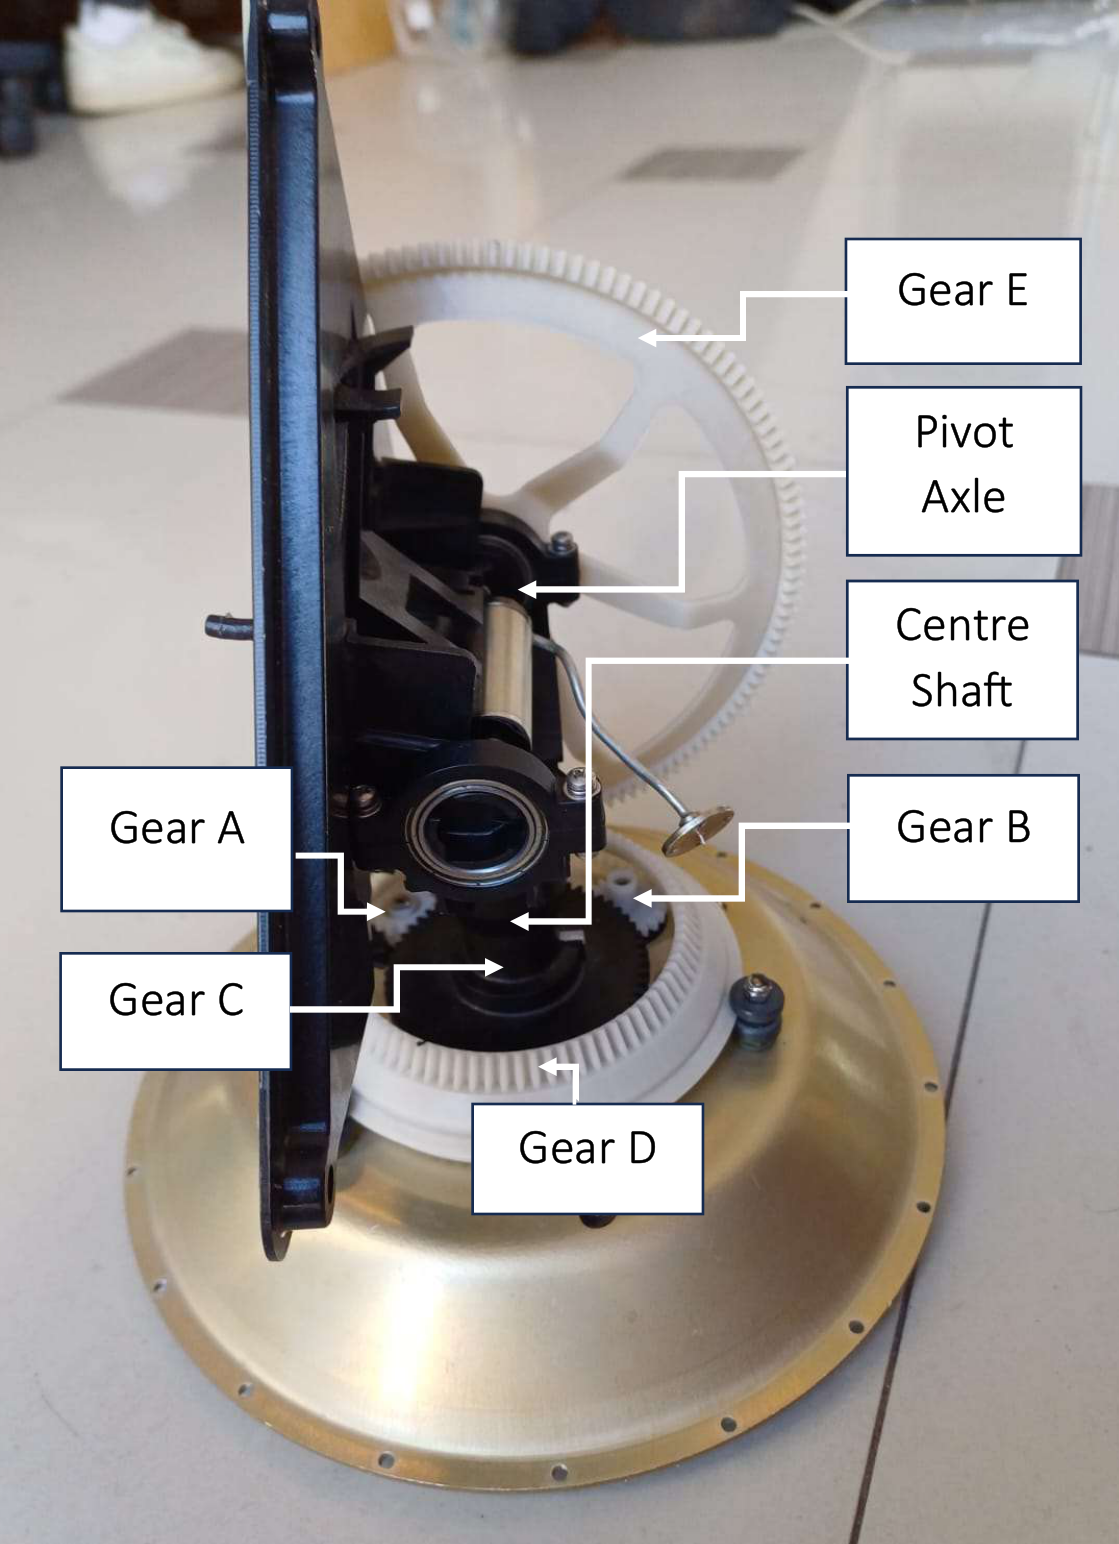
\includegraphics[width=0.35\textwidth]{antennaMount}
    \caption{The Existing Antenna Mount}
    \label{fig:antennaMount}
\end{figure}

Since stepper motors are included, the \textit{open-loop} method will be considered, however the closed loop method may be implemented if this method is found to lack accuracy, or the motor locations are found to be unpredictable, during testing. In this case, an inertial measurement unit (IMU), which typically includes an accelerometer and gyroscope, will be used.

\subsection{Monitoring}
A laptop will be used with a simple Graphical User Application (GUI) allowing the user to:
\begin{itemize}
    \item Send commands to the ground station and/or satellite.
    \item Read telemetry of the satelite.
    \item Control the ground station orientation e.g. performing motor calibration etc.
    \item Set communication parameters e.g. output power and modulation parameters.
    \item Monitor communication link performance.
\end{itemize}